\documentclass[mathserif]{beamer}
\usetheme{Luebeck}
%\usepackage[francais]{babel}
\usepackage[utf8]{inputenc} % Uses the utf8 input encoding
\usepackage[T1]{fontenc} % Use 8-bit encoding that has 256 glyphs

\usepackage[nomath]{kpfonts}
\usepackage{eulervm}
%\usepackage{default}

\usepackage{amsthm}
\usepackage{amssymb}
\usepackage{xparse}
\usepackage{thmtools}
\usepackage{stackrel}

%shortcuts
\newcommand{\R}{\mathbb{R}}
\newcommand{\C}{\mathbb{C}}
\newcommand{\Z}{\mathbb{Z}}
\newcommand{\N}{\mathbb{N}}
\newcommand{\fii}{\varphi}
\newcommand{\dd}{\mathrm{d}}
\newcommand{\CP}{\mathbb{CP}}
\renewcommand{\S}{\mathbb{S}}
\DeclareMathOperator{\Sp}{Sp}
\DeclareMathOperator{\tr}{tr}
\DeclareMathOperator{\dist}{dist}

% theorems configuration

\makeatletter
\newtheoremstyle{indented}
{7pt} %vertical space before
{7pt} % vertical space after
{} %{\addtolength{\@totalleftmargin}{2.5em}
	%\addtolength{\linewidth}{-3.5em}
	%\parshape 1 3.5em \linewidth} %body font
{1.5em} %indent
{\bfseries} %header font
{.} %punctuation
{.5em} %horizontal space after header
{} %header specification

\theoremstyle{definition}

\newtheorem{defn}{Définition}[section]

\theoremstyle{plain}
%\newtheorem*{theorem*}{Theorem}

\newtheorem{thm}{Théorème}

\renewcommand{\thetheorem}{\Alph{theorem}}
\newenvironment{preuve}{
	\noindent \textbf{Proof. }}{\hfill $\square$\medskip\par}

\newtheorem{exemple}[defn]{Example}
\newtheorem{prop}[defn]{Proposition}
\newtheorem{corr}[defn]{Corollary}
\newtheorem{por}[defn]{Porisme}
\newtheorem{ex}[defn]{Example}
\newtheorem{lem}[defn]{Lemma}
\newtheorem{conj}{Conjecture}
\newtheorem{ax}{Axiom}  %Axioms have their own numerotation

\theoremstyle{definition}
\newtheorem{rem}[defn]{Remark} %remarks are not indented
\newtheorem{rems}[defn]{Remarks}

%--------------
% Mise en page mathématique
%--------------
\addtolength{\jot}{.2em}


\title[Localization of low-energy states for Toeplitz Operators]{Localization of low-energy states for semiclassical Toeplitz Operators}
\author[Alix Deleporte]{Alix Deleporte\\Advisor : Nalini Anantharaman}
\institute[IRMA]{Institut de Recherche Mathématique
  Avancée\\Université de Strasbourg}

\AtBeginSection
{
	\begin{frame}
		\frametitle{Plan}
		\tableofcontents[currentsection]
	\end{frame}
	
}

\newcommand{\spline}{\hline}
\renewcommand{\arraystretch}{1.3}
\begin{document}
\begin{frame}
	\titlepage
\end{frame}

\begin{frame}\frametitle{Introduction}
\begin{center}
	\begin{tabular}{|c|c|}
		\spline
	    Classical mechanics & Quantum mechanics\\
		\spline
		Symplectic manifold $M$ & Hilbert Space $H$\\ 
		\spline 
		Function $a\in C^{\infty}(M,\R)$ & Self-adjoint
                                                   operator $A\in L(H)$\\
		\spline
                Hamiltonien flow of $a$ & Flow of $e^{itA/\hbar}$\\
		\spline
		Poisson Bracket & Lie Bracket\\
		\spline
	\end{tabular}\end{center}\vspace{0em}
	\begin{itemize}
	\uncover<2>{\item Quantization : for a given classical
          model, how to construct an associated quantum
          model ?
	
	\item Semiclassics : the quantum model is $\hbar$-dependent. What
          can be said in the $\hbar\to 0$ limit ?}
	\end{itemize}
\end{frame}

\begin{frame}\frametitle{Introduction}
	\begin{itemize}
		\item Quantum spins: triplet of self-adjoint matrices
                  $S_x,S_y,S_z\in M_{2S+1}(\C)$, with $$[S_a,S_b]=\frac{i}{S}\epsilon_{abc}S_c.$$
		\item For $S=\frac 12$, one finds the Pauli matrices
		$$S_x=\tiny{\frac 12\begin{pmatrix}
		0& 1\\1& 0
		\end{pmatrix}}\quad S_y=\frac 12\begin{pmatrix}
		0& i\\-i& 0
		\end{pmatrix}\quad S_z=\frac 12\begin{pmatrix}
		1& 0\\0& -1
		\end{pmatrix}.$$
		\uncover<2>{\item For any finite graph $G$, we wish to study the
                  following operator acting on $(\C^{2S+1})^{\otimes |G|}$:
		$$H=\sum_{e\sim f}S_{x,e}S_{x,f}+S_{y,e}S_{y,f}+S_{z,e}S_{z,f}$$
		as $S\to +\infty$.}
	\end{itemize}
\end{frame}

\section{Toeplitz operators on Bargmann spaces}
\subsection{Bargmann spaces}
\begin{frame}\frametitle{Bargmann spaces}
	The Bargmann spaces are $L^2$ spaces of holomorphic functions
        on $\C^n$, with a weight.
	\begin{equation*}
		B_N(\C^n)=\left\{z\mapsto \exp\left(-\frac N2|z|^2\right)f(z),\,f\text{ holomorphic}\right\}\cap L^2(\C^n)
	\end{equation*}
	Those are closed subspaces of $L^2(\C^n)$.
\end{frame}
\begin{frame}\frametitle{The Szeg\H{o} projector}
	Let $\Pi_N$ be the orthogonal projector from $L^2(\C^n)$ onto
        $B_N(\C^n)$. $\Pi_N$. It admits a Schwartz kernel:
	\begin{equation*}
		\Pi_N(z,w)=\frac{N^n}{\pi^n}\exp\left[N(-\frac 12 |z-w|^2+i\Im(z\cdot \overline{w}))\right].
	\end{equation*}
	As $N\to +\infty$, the kernel is exponentially decreasing far
        from the diagonal. The typical interaction scale is $N^{-1/2}$.
\end{frame}
\subsection{Definition}
\begin{frame}
\frametitle{Toeplitz operators}
\begin{defn}
	Let $h\in C^{\infty}(\C^n)$ a smooth bounded function, and
        $N\in \N$. We denote by $T_N(h)$ the Toeplitz operator
        associated to $h$:
	\begin{equation*}
		\begin{array}{rcl}
		T_N(h):B_N(\C^n)&\mapsto & B_N(\C^n)\\
		u& \mapsto& \Pi_N(hu).
		\end{array}
	\end{equation*}
\end{defn}
If $h$ is not bounded, we can construct $T_N(h)$ as an unbounded
operator on $B_N(\C^n)$. 

The mapping $h\mapsto T_N(h)$ is linear and adjoint-preserving. If $h$
is real-valued, then $T_N(h)$ is formally self-adjoint.
\end{frame}

\begin{frame}\frametitle{Anti-Wick quantization}
		\begin{itemize}
		\item<1-> There holds $T_N(1)=1$, and if $h$ is
                  holomorphic, then$T_N(h)=h$ ; for instance $T_N(z_i)=z_i$.
		
		\item<2-> Moreover $T_N(\overline{z}_i)=N^{-1}\partial_i.$
		
		\item<3-> If $h:z\mapsto \overline{z}^{\alpha}z^{\beta}$, then $T_N(h)=N^{-|\alpha|}\partial^{\alpha}z^{\beta}$.
		
		\item<4-> If $q$ is a definite quadratic form on 
                  $\R^{2n}$, then $T_N(q)$ has a compact
                  resolvent. The first eigenvalue
                  $\mu_N(q)=N^{-1}\mu_1(q)$ is positive.

                  \begin{equation*}
                    \mu_1(q)=\min \Sp(Op^W_1(q)) + \frac 12 \tr(q)
                  \end{equation*}
		\end{itemize}
\end{frame}

\subsection{Semiclassical properties}
\begin{frame}\frametitle{Composition and bracket}
	\begin{prop}
		Let$a$ and $b$ two smooth bounded functions on
                $\C^n$. Then there is a sequence $(c_i)_{i\in \N}$ of
                smooth bounded functions on $\C^n$, with $c_0=ab$ so
                that, as $N\to +\infty$, there holds:
		\begin{equation*}
			T_N(a)T_N(b)=T_N(c_0)+N^{-1}T_N(c_1)+N^{-2}T_N(c_2)+\ldots
		\end{equation*}
		
		\uncover<2>{In particular,
		\begin{equation*}
			[T_N(a),T_N(b)]=\cfrac{i}{N}T_N(\{a,b\})+O(N^{-2}).
		\end{equation*}}
	\end{prop}
\end{frame}

\section{Generalization to K\"ahler manifolds}
\begin{frame}
	\begin{itemize}
		\item We wish to generalize Bargmann spaces to other
                  complex manifolds.
		\item As previously, without a good choice of a
                  weight, the outcome is trivial.
		\item<2> Instead of considering weighted spaces, we
                  will consider spaces of holomorphic sections.
	\end{itemize}
\end{frame}
\subsection{Hardy spaces}
\begin{frame}\frametitle{Notations}
	\begin{itemize}
		\item $M$ is a compact K\"ahler manifold, with
                  symplectic form $\omega$.
		\item $L$ is a complex line bundle on $M$, endowed
                  with a hermitian structure $h$, so that the
                  curvature of the Chern connexion is $\omega$.
		\item $N\geq 1$ is an integer.
	\end{itemize}
	\uncover<2->{Then if $s$ is a (continuous) section of
          $L^{\otimes N}$, one can compute $$\|s\|_{L^2}:=\int_M h_N(s(m))\cfrac{\omega^{\wedge n}}{n!}.$$
	By completion, one defines the Hilbert space of square-integrable sections of $L^{\otimes N}$.}
\end{frame}

\begin{frame}\frametitle{Hardy spaces}
	\begin{defn}
		The \emph{N-equivariant Hardy space} is the space
                $H_N(M,L)$ of $L^2$ and holomorphic sections of $L^{\otimes N}$.
	\end{defn}
	This space is finite-dimensional, the dimension is polynomial
        in $N$ (Riemann-Roch).
	\uncover<2>{\begin{defn}
		The \emph{Szeg\H{o} projector} $S_N$ is
                the orthogonal projector from $L^2(M,L^{\otimes N})$ onto $H_N(M,L)$.
	\end{defn}
	It always admits a Schwartz kernel ( as a section of
        $L^{\otimes N}\boxtimes L^{\otimes -N}$) because $H_N(M,L)$ is finite-dimensional.}\end{frame}

\begin{frame}\frametitle{Toeplitz operators}
	\begin{defn}
		Let $h\in C^{\infty}(M)$ a smooth function, and $N\in
                \N$. We denote by $T_N(h)$ the Toeplitz operator
                associated with $h$:
		\begin{equation*}
		\begin{array}{rcl}
		T_N(h):H_N(M,L)&\mapsto & H_N(M,L)\\
		u& \mapsto& S_N(hu).
		\end{array}
		\end{equation*}
	\end{defn}
	$T_N(h)$ acts on a finite-dimensional space, and it is
        symmetric when $h$ is real-valued.

\uncover<2>{Observe that, for any $u,v\in H_N(M,L)$, there
  holds $$\langle u, T_N(h)v\rangle = \langle u,hv\rangle.$$}
\end{frame}
\subsection{Semiclassical properties}
\begin{frame}\frametitle{Asymptotics for the Szeg\H{o} projector}
	\begin{prop}[Boutet-Sjostrand 74]
		For every $\epsilon>0$ and $k\in \N$ there exists $C$
                such that, for every $N\in \N$:
		\begin{equation*}
			d(x,y)>\epsilon \Rightarrow |S_N(x,y)|\leq C N^{-k}
		\end{equation*}
	\end{prop}
	\uncover<2>{\begin{prop}[Charles 00, Zelditch 02, Ma 06]
		In a convenient system of local coordinates, near any
                point of the diagonal, there holds:
		\begin{equation*}
			S_N(z,w)\simeq\Pi_N(z,w)\left[1+\sum_{k=1}^KN^{-k/2}b_k(\sqrt{N}z,\sqrt{N}w)\right]
		\end{equation*}
	\end{prop}}
\end{frame}

\begin{frame}\frametitle{Composition and bracket}
	\begin{prop}[Charles 00, Schlichenmaier 02]
          Let $a$ and $b$ two smooth functions on $M$. Then
          there is a sequence $(c_i)_{i\in \N}$ of smooth functions on
           $M$, with $c_0=ab$, such that, as $N\to +\infty$, there holds:
		\begin{equation*}
		T_N(a)T_N(b)=T_N(c_0)+N^{-1}T_N(c_1)+N^{-2}T_N(c_2)+\ldots
		\end{equation*}
		
		In particular,
		\begin{equation*}
		[T_N(a),T_N(b)]=\cfrac{i}{N}T_N(\{a,b\})+O(N^{-2}).
		\end{equation*}
	\end{prop}
\end{frame}
\subsection{An example: the sphere}
\begin{frame}\frametitle{Hardy spaces on the sphere}
	\begin{itemize}
	\item $H_N(\CP^1,L)$ corresponds to the the set of meromorphic
          functions on the sphere, with one pole of order at most $N$.
	
	\item Hence $H_N(\CP^1,L)\simeq \C_{N}[X]$, with dimension $N+1$.
	
	\item One Hilbert base is:
	$$e_{k,N}(X)=\frac{\binom{k}{N}^{1/2}}{N}X^k.$$
	\end{itemize}
\end{frame}

\begin{frame}
	\frametitle{Coordinate functions}
	\begin{minipage}{0.44\linewidth}
	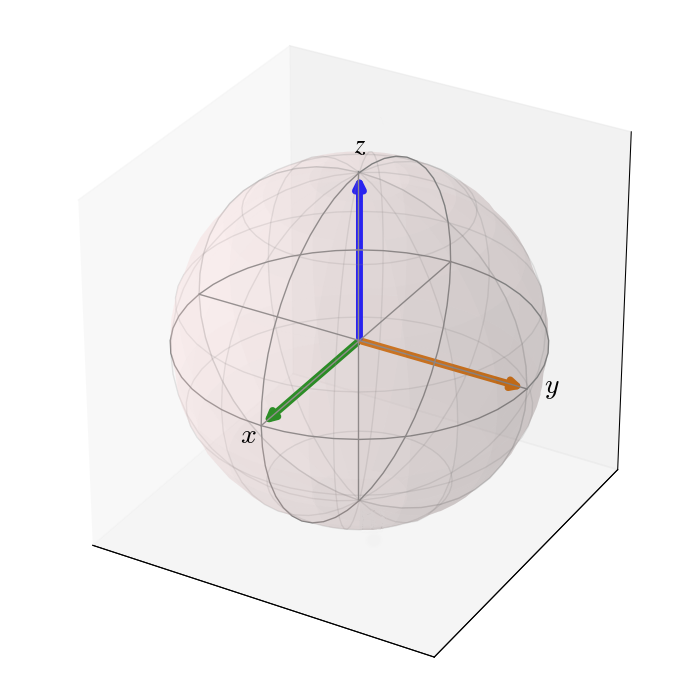
\includegraphics[scale=0.3]{sphere.png}
	\end{minipage}
	\begin{minipage}{0.55\linewidth}
	\begin{itemize}
			\item There are three coordinate functions on
                          the sphere: $x$, $y$ and $z$.
	\item The Toeplitz quantizations of these three functions are
          the spin operators, with $S=\frac{N}{2}$.
	\end{itemize}\end{minipage}
\end{frame}

\section{The smallest eigenvalue}
\begin{frame}\frametitle{A priori localization}
	\begin{itemize}
		\item In the classical model, in order to minimize the
                  energy, one picks any point where the energy is minimal.
		\item What happens for an eigenvector associated with
                  the smallest eigenvalue of $T_N(h)$, as $N\to +\infty$ ?
	\end{itemize}
	\only<1>{\begin{prop}[Charles 00]
		An eigenvector with minimal eigenvalue is
                uniformly $O(N^{-\infty})$ outside any fixed
                neighbourhood of $\{h=min(h)\}$.
	\end{prop}
Can we get a more precise result?}
	\only<2>{\begin{prop}[D. 16]
            If the minimal set is non-degenerate, then for every
            $\delta\in [0,1/2)$, an eigenvector with minimal
            eigenvalue is uniformly $O(N^{-\infty})$ outside a
            neighbourhood of $\{h=min(h)\}$ with size $N^{-\delta}$.
	\end{prop}}

\end{frame}

\begin{frame}
  \frametitle{Proof for localization speed}
  Let $(u_N)$ be a sequence of unit eigenfunctions with minimal
  energy $(\lambda_N)$. Assume $\min(h)=0$.

  We prove by induction on $k$ that $$\langle u_n,h^ku_n\rangle =
  O(N^{-k}).$$\vspace{-2em}
  \begin{itemize}
  \uncover<2->{\item Hard part: $k=1$ (test $T_N(h)$ against a coherent state centred on
  a minimal point).}

  \uncover<3>{\item Easy part: induction. $$\langle u_n,h\star h u_n\rangle =
  \lambda_N^2 + O(N^{-\infty}),$$ where $h\star h = h^2+N^{-1}c_1(h,h)+ O(N^{-2})$.

  Now $c_1(h,h)\leq Ch$.}\end{itemize}
\end{frame}
\subsection{Wells}
\begin{frame}
  \frametitle{Case of several wells}
  \begin{minipage}[l]{0.3\linewidth}
    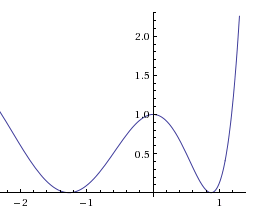
\includegraphics[width=\linewidth]{wells.png}
  \end{minipage}
  \begin{minipage}[r]{0.65\linewidth}
    What can be said if $h$ is minimal on non-degenerate critical
    points?
    
    \uncover<2->{
      \begin{thm}[D. 16]
        The eigenvectors of minimal eigenvalue concentrate only on
        ``minimal'' points. Eigenvectors and eigenvalue have an
        asymptotical expansion.
      \end{thm}
    }

    \uncover<3>{What is minimized ? The $\mu_1$ of the hessian at this
      point.}
  \end{minipage}
\end{frame}

\begin{frame}
  \frametitle{Case of wells: idea of proof}
  \begin{itemize}
  \item By making more precise the previous argument, we have a lower
    bound for the first eigenvalue.
  \item The upper bound and a spectral gap are obtained by
    $N^{-K}$-quasimode for fixed $K$.
  \end{itemize}

We remark that the quasimodes are exponentially localized, but this
does not imply that the true eigenfunction is also localized.
\end{frame}

\subsection{Miniwells}

\begin{frame}
  \frametitle{Case of submanifold wells}
  \begin{itemize}
\item What can be said if $h$ is minimal on a submanifold, with
  non-degenerate transverse hessian?
  \item $\Rightarrow$ Same conclusion. (D.)\end{itemize}
   \begin{minipage}[l]{0.3\linewidth}
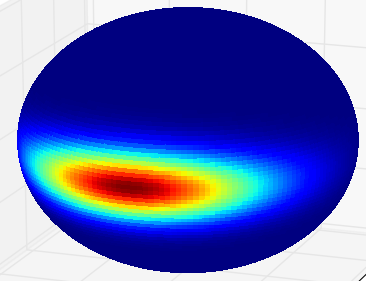
\includegraphics[scale=0.3]{35.png}\end{minipage}\begin{minipage}[r]{0.65\linewidth}
As $N$ grows, the state concentrates on the miniwell and is more
and more squeezed.\end{minipage}
\end{frame}
\begin{frame}
\frametitle{Miniwells in physics}
    It really happens in physics ! For instance, with
      antiferromagnetic spins on a triangle graph.
\begin{minipage}[l]{0.3\linewidth}
      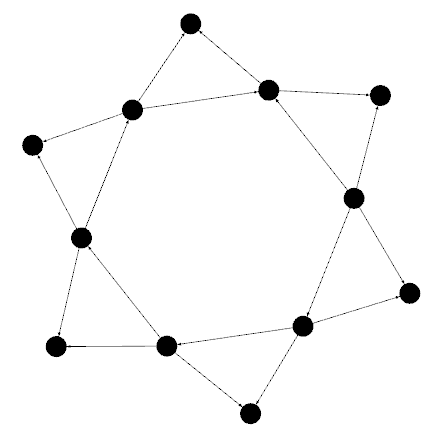
\includegraphics[scale=0.2]{hexa.png}\end{minipage}\begin{minipage}[r]{0.65\linewidth}
      It is conjectured that the minimal configurations are planar, in
      some cases.
      \end{minipage}

\end{frame}
\subsection{Conjectures}
\begin{frame}
  \frametitle{Conjectures}
  \begin{description}
  \item[Exponential Localization] For now we only have
    $O(N^{-\infty})$ estimates for localisation. Can we hope for
    $O(\exp(-cN))$ estimates ?
  \item[Thermodynamical limit] Instead of considering a fixed manifold
    $M$, we look at a particular symbol on $M^n$, and we let $n\to
    +\infty$. What is the behaviour vis-à-vis the semiclassical limit?
  \end{description}

These two questions should be linked with each other.
\end{frame}
\end{document}